%%%%%%%%%%%%%%%%%%%%%%%%%%%%%%%%%%%%%%%%%%%%%%%%%%%%%%%%%%%%%%%%%%%%%%%%%%%%%%%%
\chapter{Introduction and Motivation}
\label{chap:introduction}

Modern Radio Access Network (RAN) optimization has traditionally relied on manual inspection of vast performance datasets, reactive troubleshooting workflows, and fragmented software tooling. As LTE and 5G New Radio (NR) networks continue to expand in scale and operational complexity, this approach becomes increasingly inefficient, inconsistent, and incapable of delivering timely engineering decisions. This graduation project presents \textbf{RANPilotAI}, an integrated, AI-powered platform designed to automate and augment the daily workflows of Radio Frequency (RF) optimization engineers in 4G LTE and 5G mobile networks.

The platform unifies four specialized analytical modules within a single web-based environment called the \textbf{Telecom Hub}, implemented using the Streamlit framework. The developed modules address the complete RAN optimization cycle: the \textbf{KPI Degradation Analyzer} detects and classifies performance degradations using statistically rigorous methods; the \textbf{KPI Forecasting Engine} predicts future network performance trajectories using ensemble time-series models; the \textbf{Optimization Action Analyzer} correlates configuration changes with KPI impact using version-controlled data management; and the \textbf{Telecom RAG Assistant} enables natural-language consultation of official 3GPP Technical Specifications through Retrieval-Augmented Generation.

%%%%%%%%%%%%%%%%%%%%%%%%%%%%%%%%%%%%%%%%%%%%%%%%%%%%%%%%%%%%%%%%%%%%%%%%%%%%%%%%
\section{Introduction}

Modern telecommunications networks generate extraordinary volumes of performance management data. A single LTE macro cell produces thousands of performance counter records every hour, spanning dozens of Key Performance Indicator (KPI) categories including accessibility, retainability, mobility, integrity, and availability metrics \cite{sesia2011}. For a metropolitan network comprising thousands of cells, this results in datasets containing millions of rows and hundreds of columns that must be analysed daily to maintain acceptable subscriber quality of service.

The traditional approach to network optimization relies on human engineers manually inspecting these datasets, applying domain expertise to identify degraded cells, determining probable root causes, and recommending corrective actions. While effective for small networks, this workflow does not scale to modern network sizes. An engineer manually reviewing a weekly KPI report for a city-scale deployment may spend hours identifying cells requiring attention, and the consistency of the analysis depends entirely on the individual engineer's experience and concentration \cite{holma2011}.

Figure~\ref{fig:ranpilotai_home} presents the home interface of the RANPilotAI platform. The interface provides centralized access to all four analytical modules through the Telecom Hub, presenting each module as a selectable capability card alongside platform information and navigation controls.

\begin{figure}[H]
    \centering
    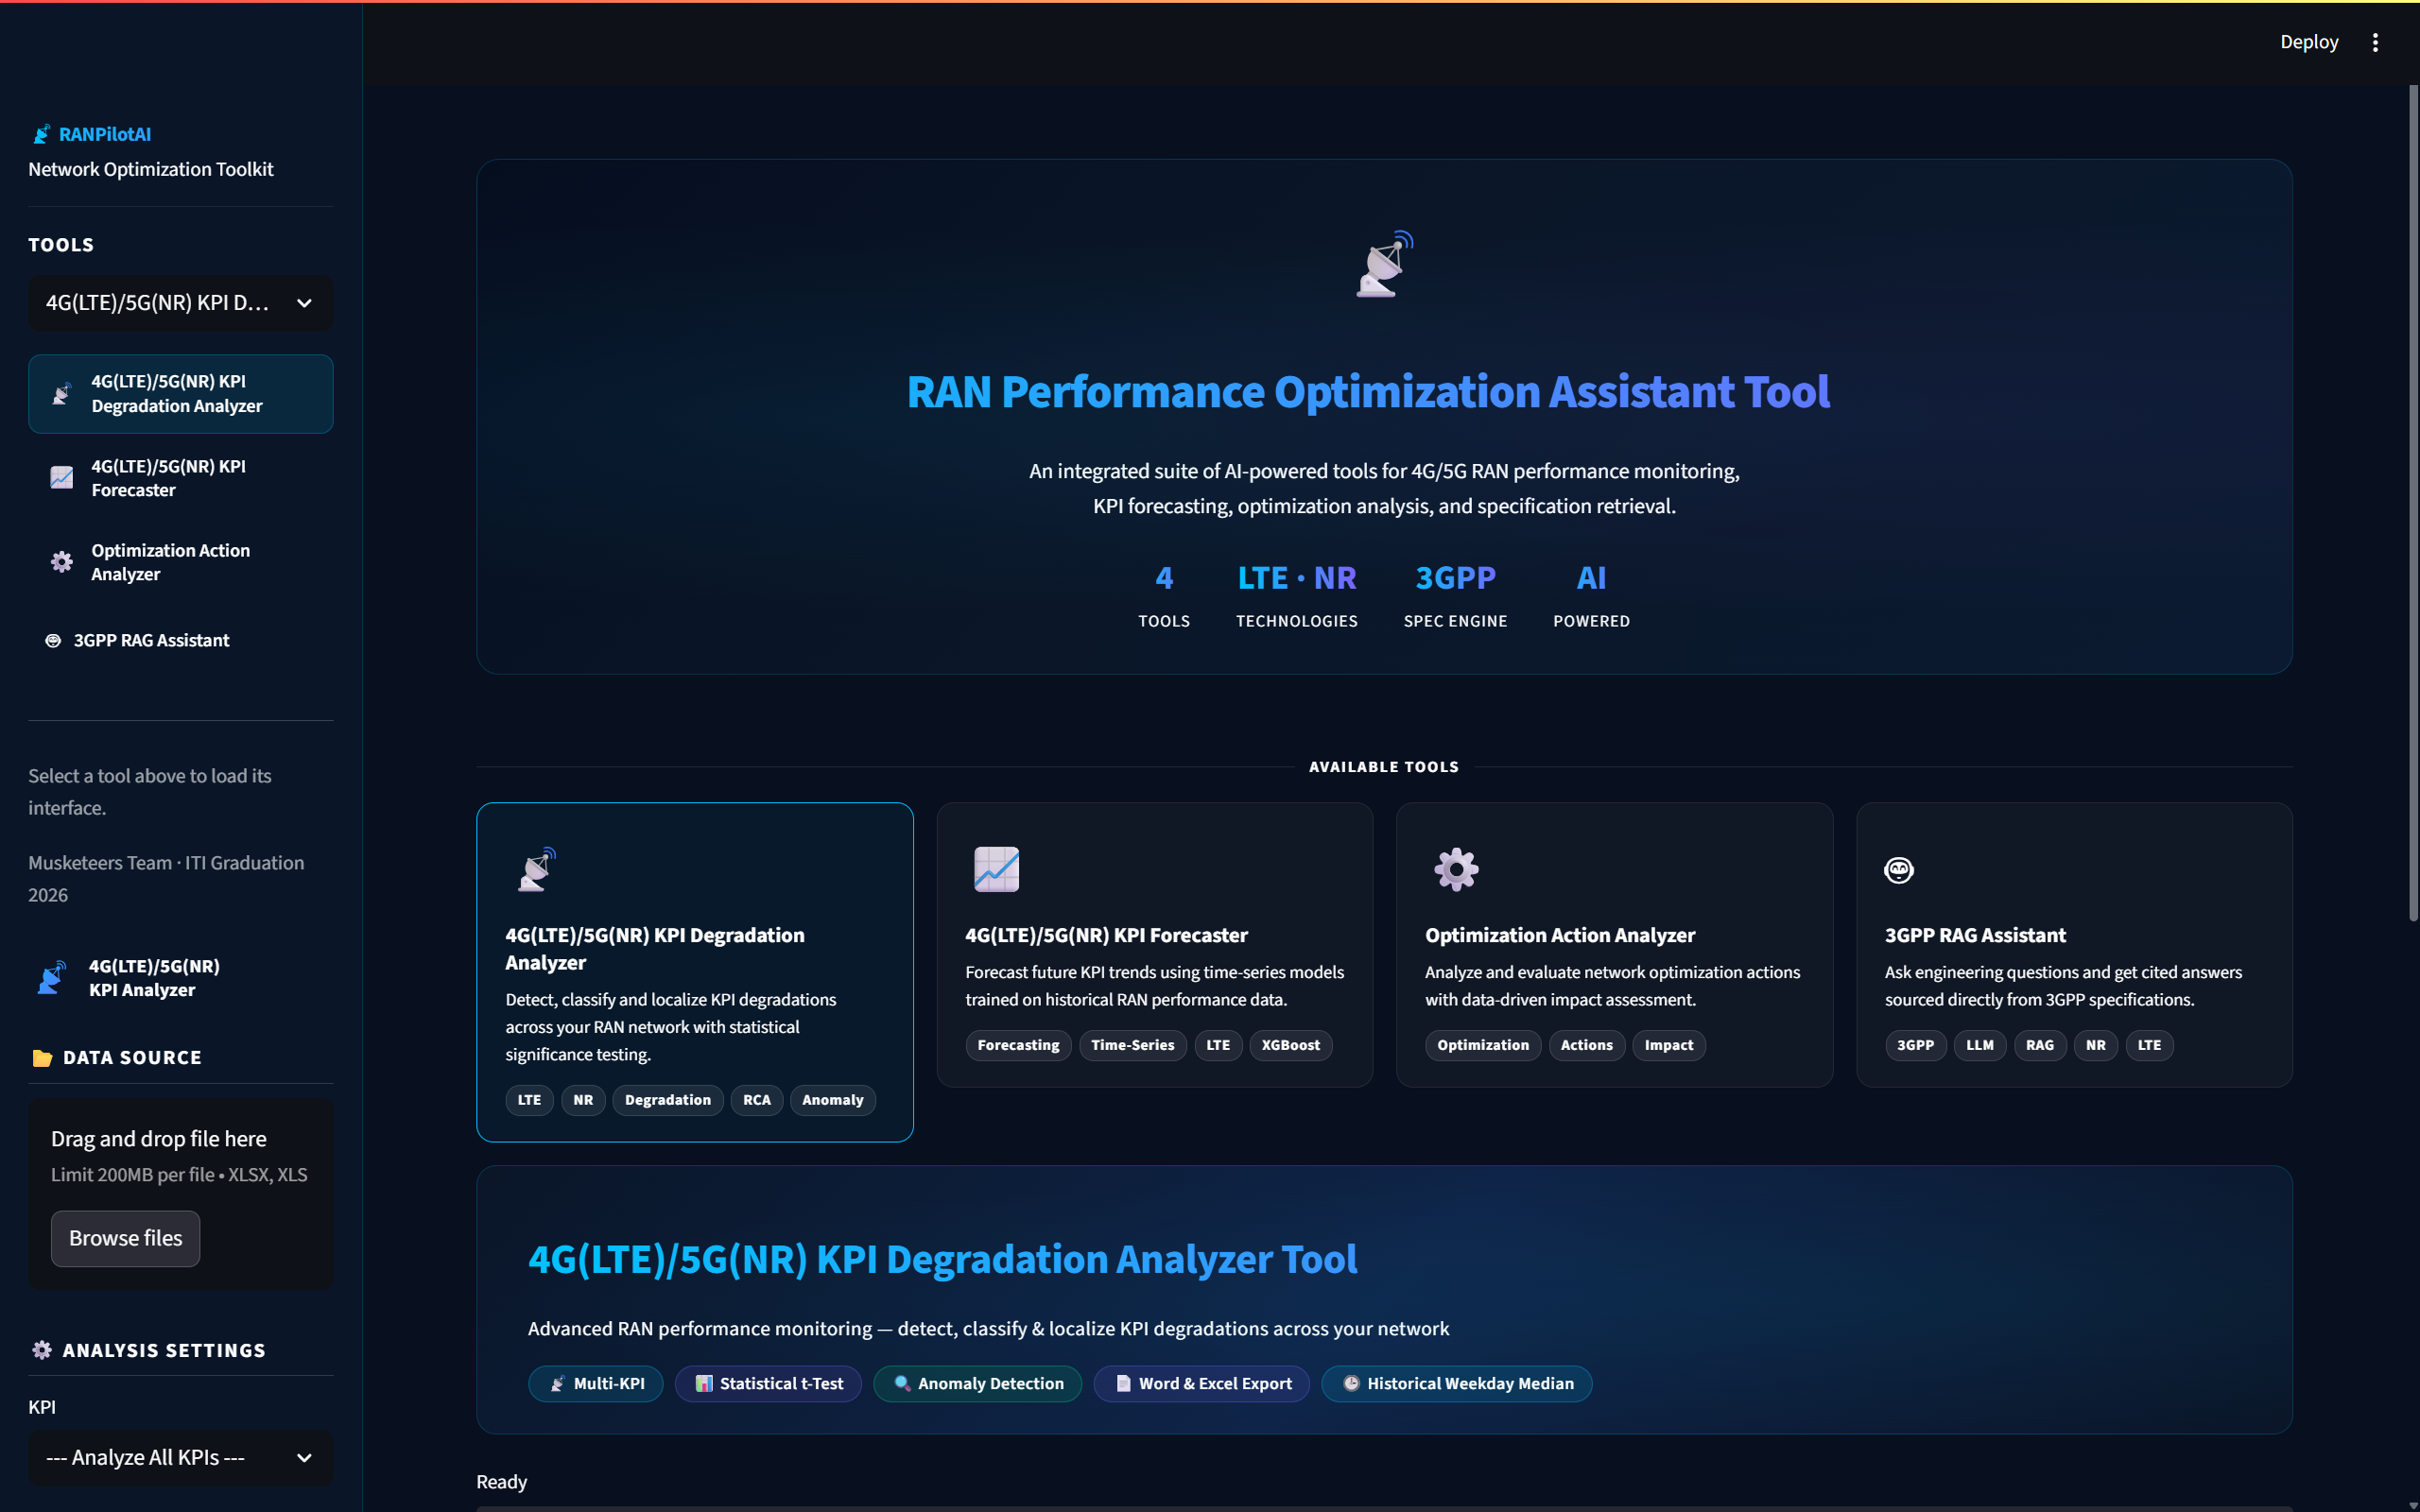
\includegraphics[width=\textwidth]{figures/chapter01/ranpilotai_home.png}
    \caption{Home interface of the RANPilotAI platform presenting the Telecom Hub with the four selectable analytical modules: KPI Degradation Analyzer, KPI Forecasting Engine, Optimization Action Analyzer, and Telecom RAG Assistant.}
    \label{fig:ranpilotai_home}
\end{figure}

The platform architecture follows a modular design in which each analytical module encapsulates its own processing logic while sharing common infrastructure services provided by the Telecom Hub. Engineers interact exclusively with the hub, which manages application routing, session handling, and data persistence. This unified environment eliminates the need to switch between separate software tools during the optimization workflow, reducing context-switching overhead and ensuring that data and analysis artefacts remain accessible across modules.

%%%%%%%%%%%%%%%%%%%%%%%%%%%%%%%%%%%%%%%%%%%%%%%%%%%%%%%%%%%%%%%%%%%%%%%%%%%%%%%%
\section{Motivation}

The motivation for developing the RANPilotAI platform arises from five converging pressures in modern network operations.

First, data volume growth has outpaced manual analysis capacity. LTE and 5G NR networks produce performance counters at intervals as short as 15 minutes, generating datasets that are impractical to review manually at network scale. A mid-sized operator managing ten thousand cells across multiple frequency layers may collect over one hundred thousand KPI observations per day, a volume that defies spreadsheet-based inspection.

Second, operational tempo has accelerated. Subscriber expectations for uninterrupted service, combined with competitive pressure and regulatory service-level obligations, require network issues to be identified and resolved within hours rather than days. Reactive workflows that detect degradation only after subscriber complaints or quality-of-service breaches are no longer acceptable.

Third, domain expertise is becoming scarce. The retirement of experienced RF engineers who accumulated decades of hands-on network knowledge creates a skills gap that manual troubleshooting workflows cannot bridge. Systematic, knowledge-encoded automation is required to preserve and transfer this expertise to new engineering teams.

Fourth, existing tooling is fragmented. Network optimization currently requires engineers to interact with multiple vendor-specific network management systems, spreadsheet applications, statistical packages, and documentation repositories. The absence of a unified environment increases cognitive load, introduces data transfer errors, and fragments the audit trail of engineering decisions.

Fifth, artificial intelligence technologies have matured to the point where they can reliably assist with domain-specific engineering tasks. Advances in statistical learning, gradient boosting, retrieval-augmented generation, and version-controlled data management provide the technical foundation for building intelligent assistance tools that are trustworthy enough for professional engineering use.

RANPilotAI was therefore conceived as a response to these pressures: a unified platform that encodes RF optimization knowledge into automated analytical modules while preserving the engineer's role as the final decision-maker. Rather than replacing engineering judgement, the platform accelerates the path from raw data to actionable insight.

%%%%%%%%%%%%%%%%%%%%%%%%%%%%%%%%%%%%%%%%%%%%%%%%%%%%%%%%%%%%%%%%%%%%%%%%%%%%%%%%
\section{Problem Statement}

The central problem addressed by this graduation project can be decomposed into four interrelated technical challenges.

\textbf{Scalable degradation detection}: Network operators require automated methods for identifying performance degradations across thousands of cells and dozens of KPI categories without manual threshold tuning or cell-by-cell inspection. The detection method must account for the natural variability of each cell's historical performance, handle data quality artefacts introduced by vendor systems, and assign statistically meaningful confidence levels to detected degradations.

\textbf{Predictive performance modelling}: Reactive maintenance — addressing network issues only after they manifest as subscriber-facing incidents — is costly and operationally undesirable. Operators need reliable forecasts of future KPI trajectories to enable proactive interventions. Forecasting must accommodate non-linear temporal dependencies, multi-KPI interactions, and varying degrees of seasonality across different cells and KPIs.

\textbf{Optimization impact quantification}: RF configuration changes — including antenna tilt adjustments, transmit power modifications, and handover parameter updates — produce effects that are difficult to isolate from normal network variability. Engineers require systematic methods for correlating configuration commits with KPI changes while controlling for confounding factors such as traffic patterns, weather, and concurrent network events.

\textbf{Standards consultation efficiency}: 3GPP Technical Specifications contain thousands of pages of protocol definitions, signaling procedures, and configuration parameters distributed across hundreds of documents. Engineers require efficient mechanisms for locating and interpreting relevant standards content without spending hours navigating PDF files or relying on potentially inaccurate memory.

%%%%%%%%%%%%%%%%%%%%%%%%%%%%%%%%%%%%%%%%%%%%%%%%%%%%%%%%%%%%%%%%%%%%%%%%%%%%%%%%
\section{Background}

\subsection{Radio Access Network Performance Management}

A Radio Access Network connects user equipment — mobile phones, IoT devices, and other wireless terminals — to the mobile core network through base stations known as evolved Node Bs (eNodeBs) in LTE and gNodeBs (gNBs) in 5G NR. Each base station serves one or more cells, and each cell is characterised by a set of Key Performance Indicators that quantify its operational health from multiple perspectives \cite{dahlman2020}.

The three primary performance pillars used in RAN assessment are accessibility, retainability, and mobility. Accessibility measures the ability of user equipment to establish connections, quantified through indicators such as RRC Setup Success Rate and E-RAB Setup Success Rate. Retainability measures the ability to maintain established connections, quantified through E-RAB Drop Rate and RRC Re-establishment Success Rate. Mobility measures the success of handover procedures between cells, quantified through Handover Success Rate and RRC Re-establishment delay \cite{sesia2011}.

In addition to these core pillars, modern networks monitor throughput KPIs (DL/UL Traffic Volume and Throughput), availability metrics (Cell Availability and Downtime), and service-specific indicators for VoLTE and CSFB services. Table~\ref{tab:kpi_pillars} summarises the five standard performance pillars and their associated KPI categories.

\begin{table}[H]
    \centering
    \caption{Standard RAN performance pillars and associated KPI categories monitored by the RANPilotAI platform.}
    \label{tab:kpi_pillars}
    \begin{tabular}{|l|p{8cm}|}
        \hline
        \textbf{Pillar} & \textbf{Associated KPI Categories} \\
        \hline
        Accessibility & RRC Setup Success Rate, E-RAB Setup Success Rate, RACH Success Rate, CSFB KPIs \\
        \hline
        Retainability & E-RAB Drop Rate, RRC Re-establishment Success Rate \\
        \hline
        Mobility & Handover Success Rate \\
        \hline
        Integrity & DL Throughput, UL Throughput, VoLTE KPIs \\
        \hline
        Availability & Cell Availability, Downtime \\
        \hline
    \end{tabular}
\end{table}

\subsection{Network Optimization Workflow}

The standard network optimization workflow comprises four phases: data collection, performance analysis, root cause identification, and corrective action implementation. In the data collection phase, network management systems export performance counter data at regular intervals, typically every 15 minutes for LTE networks and every 5 minutes for 5G NR networks. This data is stored in proprietary vendor formats and must be transformed into analysis-ready tabular structures before statistical processing can begin.

The performance analysis phase involves identifying cells whose KPI values have degraded relative to their historical baselines. Engineers apply thresholds — often fixed values inherited from vendor recommendations — to flag underperforming cells. Threshold-based alerting suffers from high false-positive rates because it ignores the natural variability and baseline performance level of each individual cell \cite{mishra2007}.

The root cause identification phase requires the engineer to examine the diagnostic counters associated with each flagged cell and apply domain knowledge to determine the probable cause of degradation. Common root causes include coverage problems (insufficient signal strength or excessive interference), capacity congestion (insufficient resources relative to traffic demand), hardware faults, and configuration errors \cite{holma2011}.

The corrective action phase involves implementing configuration changes — such as adjusting antenna tilt, modifying handover parameters, or adding capacity — and then monitoring the resulting KPI impact to validate the intervention.

%%%%%%%%%%%%%%%%%%%%%%%%%%%%%%%%%%%%%%%%%%%%%%%%%%%%%%%%%%%%%%%%%%%%%%%%%%%%%%%%
\section{Proposed Solution Overview}

RANPilotAI addresses the limitations of manual network optimization by encoding each phase of the workflow into dedicated analytical modules implemented within a unified web-based platform. The platform operates as a centralized engineering environment accessible through a standard web browser, eliminating the need for client-side software installation and enabling engineers to perform complex analytical tasks from any workstation.

The platform architecture follows a modular design philosophy in which the Telecom Hub acts as the central coordination point. Rather than exposing individual module interfaces directly to the user, the hub provides a consistent navigation paradigm, shared session management, and common data services. Each module communicates with the hub through standardized interfaces, preserving module autonomy while ensuring data consistency across the platform.

The technical implementation adopts Python 3.11 as the primary development language, with Streamlit providing the web-based user interface framework. Data processing leverages the Pandas and NumPy scientific computing ecosystem, while machine learning components are built upon Scikit-learn, XGBoost, and Statsmodels. Retrieval-augmented generation capabilities are provided through sentence-transformers, Qdrant vector database, and OpenRouter language model APIs. Version-controlled data management is provided through Dolt, a SQL database with Git-like versioning semantics.

%%%%%%%%%%%%%%%%%%%%%%%%%%%%%%%%%%%%%%%%%%%%%%%%%%%%%%%%%%%%%%%%%%%%%%%%%%%%%%%%
\section{Platform Modules}

The RANPilotAI platform integrates four analytical modules, each addressing a distinct phase of the RAN optimization workflow.

\subsection{KPI Degradation Analyzer}

The KPI Degradation Analyzer is the primary performance analysis module of the platform. It processes raw KPI counter exports and applies a three-layer analytical pipeline comprising data quality validation, statistical degradation detection, and RF-aware root cause analysis. The module monitors 13 KPI categories across five performance pillars and produces structured degradation reports including severity classifications, confidence scores, root cause pattern identifications, and recommended next investigation steps.

\subsection{KPI Forecasting Engine}

The KPI Forecasting Engine predicts future network performance using an ensemble of statistical and machine learning models. The module implements Holt-Winters exponential smoothing for classical seasonal pattern capture and XGBoost gradient boosting with leakage-safe cross-KPI feature engineering for non-linear multivariate modelling. A unified evaluation framework compares all candidate models against hold-out data and automatically recommends the most reliable predictor on a per-cell, per-KPI basis. The engine generates recursive 7-day forward forecasts accompanied by residual diagnostics and seasonality quantification.

\subsection{Optimization Action Analyzer}

The Optimization Action Analyzer correlates RF configuration changes with KPI impact using Dolt as a version-controlled data backend. The module tracks antenna tilt, transmit power, and other configuration parameters through commit history, aligns configuration events with KPI time windows using weekday-matched baseline comparison, and presents results through interactive timeline, before/after overlay, delta bar, and summary impact visualizations.

\subsection{Telecom RAG Assistant}

The Telecom RAG Assistant enables engineers to query official 3GPP Technical Specifications using natural language. The system combines PDF processing, section-aware chunking, BGE-large dense embeddings, local Qdrant vector search, cross-encoder re-ranking, and strict anti-hallucination prompt engineering to produce traceable, citation-backed answers grounded directly in official standards documentation.

%%%%%%%%%%%%%%%%%%%%%%%%%%%%%%%%%%%%%%%%%%%%%%%%%%%%%%%%%%%%%%%%%%%%%%%%%%%%%%%%
\section{Summary}

This chapter has introduced the RANPilotAI platform as an integrated, AI-powered solution for Radio Access Network optimization. The chapter has motivated the development of the platform through an analysis of the limitations inherent in current manual network optimization workflows, formulated the technical challenges addressed by the developed modules, and provided a high-level overview of the platform architecture and its four constituent analytical modules.

The subsequent chapters develop the platform components in detail. Chapter~\ref{chap:literature_review} surveys the relevant research literature spanning network performance management, statistical learning, time-series forecasting, root cause analysis, retrieval-augmented generation, and software architecture. Chapter~\ref{chap:system_design} presents the detailed system design, including the platform architecture, technology stack, data management strategy, and module integration interfaces. Chapters~\ref{chap:kpi_degradation} through~\ref{chap:telecom_rag} describe each analytical module in depth, following the structure established in this chapter: module introduction, operational motivation, technical problem formulation, background theory, configuration and results presentation, and summary.
